\documentclass[border=12pt]{standalone}
\def\pgfsysdriver{pgfsys-dvisvgm.def}
\usepackage[dvisvgm]{xcolor}
\usepackage{xeCJK}
\setCJKmainfont{HaranoAjiGothic-Regular.otf}[BoldFont=HaranoAjiGothic-Bold.otf]
\setCJKsansfont{HaranoAjiGothic-Regular.otf}[BoldFont=HaranoAjiGothic-Bold.otf]
\usepackage{amsmath,amssymb,tikz,lmodern}
\usetikzlibrary{arrows.meta,positioning,calc,fit,backgrounds}
\renewcommand{\familydefault}{\sfdefault}
\definecolor{ink}{HTML}{25322F}
\definecolor{green}{HTML}{246657}
\definecolor{tint}{HTML}{EEF4F0}
\definecolor{soft}{HTML}{C6D2CC}
\definecolor{muted}{HTML}{52615B}
\newif\ifJapanese
\newcommand{\Tx}[2]{\ifJapanese #1\else #2\fi}
\newcommand{\Eff}{\overline{\operatorname{Eff}}}
\newcommand{\heading}[3]{{\color{green}\bfseries #1\quad\Tx{#2}{#3}}\\[5pt]}
% A white rectangle makes the complete citation label clickable, including spaces.
\newcommand{\refurl}[2]{\special{dvisvgm:raw <a xlink:href="#1" target="_blank" rel="noopener noreferrer">}{\setlength{\fboxsep}{0pt}\colorbox{white}{\color{green}\underline{\strut #2}}}\special{dvisvgm:raw </a>}}
\newcommand{\refedge}[3]{\refurl{\csname source#1\endcsname\string##page=#2}{#3}}
\newcommand{\SF}[2]{\refedge{sf}{#1}{#2}}
% GitHub's file preview does not support PDF page fragments.
\newcommand{\LA}[2]{\refurl{\sourcela}{#2}}
\newcommand{\Sch}[2]{\refedge{sch}{#1}{#2}}
\newcommand{\PS}[2]{\refedge{ps}{#1}{#2}}
\tikzset{
 card/.style={draw=soft,fill=white,rounded corners=2pt,align=left,text=ink,font=\fontsize{10.5}{14}\selectfont,inner xsep=12pt,inner ysep=10pt,text width=14.4cm},
 half/.style={card,text width=6.45cm,minimum height=2.05cm},
 result/.style={card,draw=green,fill=tint,line width=.9pt},
 reason/.style={align=left,text=muted,font=\fontsize{9}{12}\selectfont,inner sep=0pt,text width=12.7cm},
 branchreason/.style={reason,text width=5.95cm},
 edge/.style={-{Stealth[length=2.4mm]},draw=green,line width=1pt},
 wire/.style={draw=green,line width=1pt},
}
% Keep the arrow in a dedicated left gutter; explanations never cover it.
\newcommand{\flow}[3]{
 \coordinate (#2-from) at ($(#1.south)+(-6.9,0)$);
 \coordinate (#2-to) at ($(#2.north)+(-6.9,0)$);
 \draw[edge] (#2-from)--(#2-to);
 \node[reason,anchor=west] (#2-reason) at ($(#2-from)!.5!(#2-to)+(.55,0)$) {#3};
}
\newcommand{\Cite}[2]{\refurl{\csname source#1\endcsname}{#2}}

\Japanesefalse
\newcommand{\sourcemm}{https://github.com/openai/math/blob/adc7f1241b42e322a6451854ab7e4b4c146bf78a/preprints/Minimal-metrics-and-interior-injectivity-for-nef-adjoints-September-27-2026/paper.pdf}
\newcommand{\sourcefuj}{https://ems.press/content/serial-article-files/41145}
\newcommand{\sourcedem}{https://www-fourier.univ-grenoble-alpes.fr/~demailly/manuscripts/analmeth_book.pdf}
\newcommand{\sourcelp}{https://arxiv.org/pdf/1809.02500v4}
\newcommand{\sourcegm}{https://www.numdam.org/item/10.24033/asens.2325.pdf}
\begin{document}
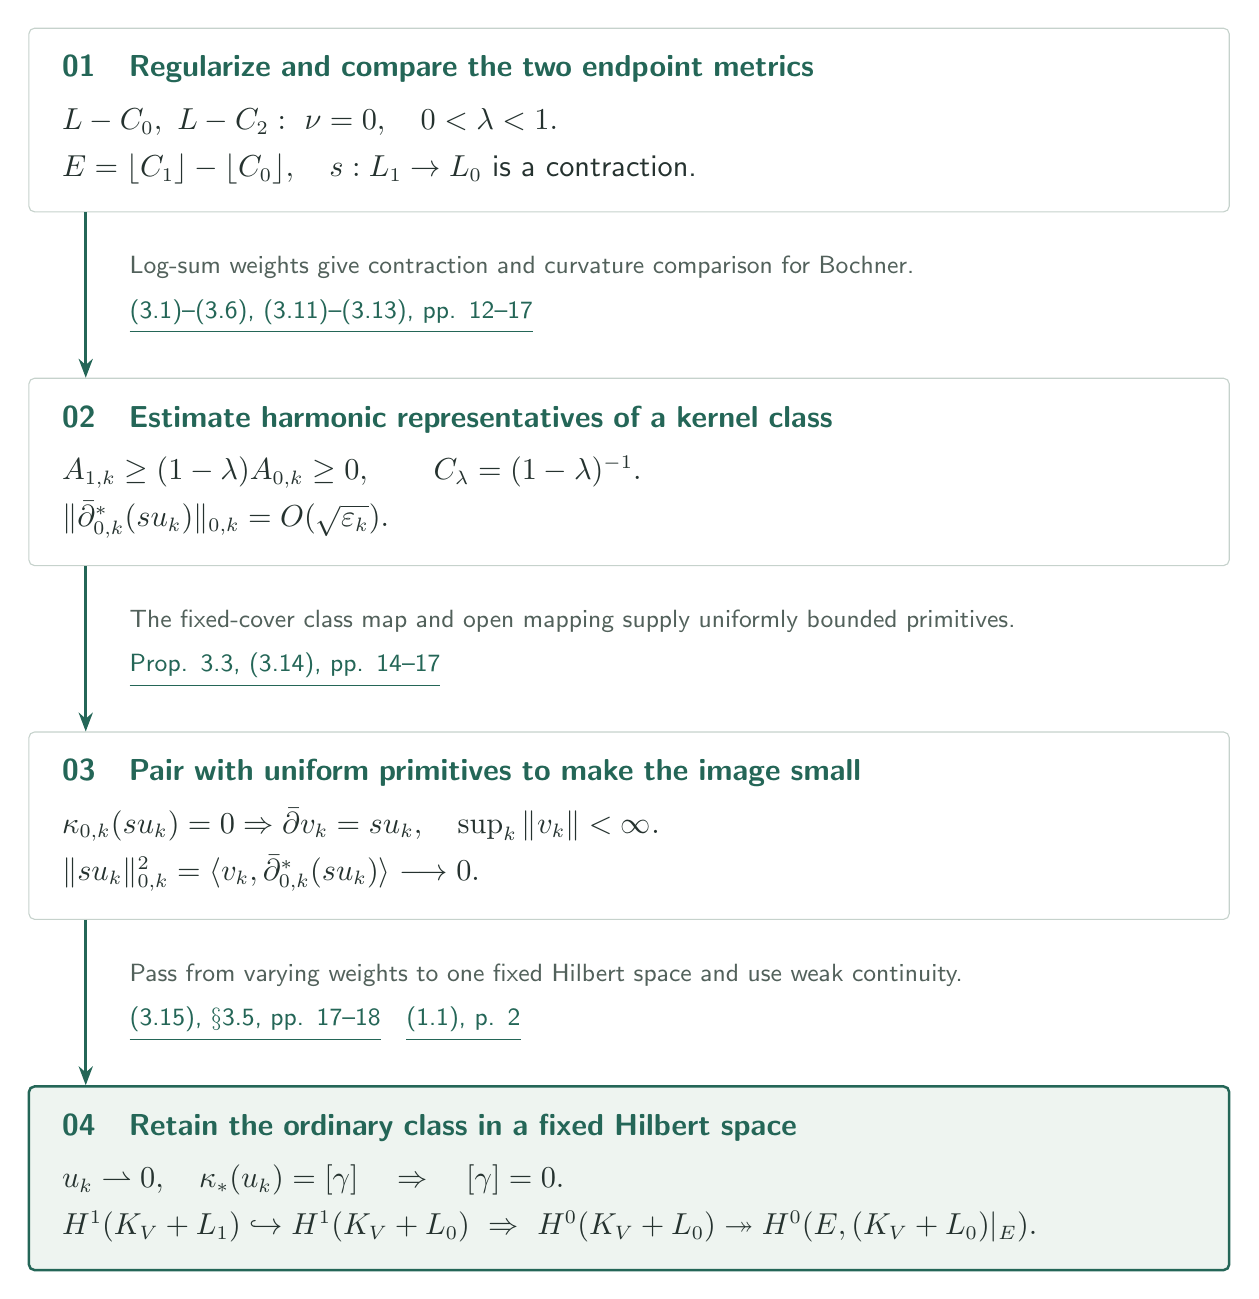
\begin{tikzpicture}
\node[card] (n0) {\heading{01}{二つの端点計量を正則化して比較する}{Regularize and compare the two endpoint metrics}\Tx{$L-C_0,\ L-C_2:\ \nu=0,\quad 0<\lambda<1.$\\[3pt]$E=\lfloor C_1\rfloor-\lfloor C_0\rfloor,\quad s:L_1\to L_0\text{ は縮小写像。}$}{$L-C_0,\ L-C_2:\ \nu=0,\quad 0<\lambda<1.$\\[3pt]$E=\lfloor C_1\rfloor-\lfloor C_0\rfloor,\quad s:L_1\to L_0\text{ is a contraction.}$}};
\node[card,below=2.1cm of n0] (n1) {\heading{02}{核の類の調和代表を評価する}{Estimate harmonic representatives of a kernel class}\Tx{$A_{1,k}\ge(1-\lambda)A_{0,k}\ge0,\qquad C_\lambda=(1-\lambda)^{-1}.$\\[3pt]$\|\bar\partial_{0,k}^*(su_k)\|_{0,k}=O(\sqrt{\varepsilon_k}).$}{$A_{1,k}\ge(1-\lambda)A_{0,k}\ge0,\qquad C_\lambda=(1-\lambda)^{-1}.$\\[3pt]$\|\bar\partial_{0,k}^*(su_k)\|_{0,k}=O(\sqrt{\varepsilon_k}).$}};
\flow{n0}{n1}{\Tx{log-sum重みで縮小性と曲率比較を両立させ、完備計量上でBochnerを使う。}{Log-sum weights give contraction and curvature comparison for Bochner.}\\[4pt]\Cite{mm}{(3.1)--(3.6), (3.11)--(3.13), pp. 12--17}}
\node[card,below=2.1cm of n1] (n2) {\heading{03}{一様な原始形と対にして像を消す}{Pair with uniform primitives to make the image small}\Tx{$\kappa_{0,k}(su_k)=0\Rightarrow\bar\partial v_k=su_k,\quad\sup_k\|v_k\|<\infty.$\\[3pt]$\|su_k\|_{0,k}^2=\langle v_k,\bar\partial_{0,k}^*(su_k)\rangle\longrightarrow0.$}{$\kappa_{0,k}(su_k)=0\Rightarrow\bar\partial v_k=su_k,\quad\sup_k\|v_k\|<\infty.$\\[3pt]$\|su_k\|_{0,k}^2=\langle v_k,\bar\partial_{0,k}^*(su_k)\rangle\longrightarrow0.$}};
\flow{n1}{n2}{\Tx{固定被覆の類写像と開写像定理で、核に一様有界な原始形を供給する。}{The fixed-cover class map and open mapping supply uniformly bounded primitives.}\\[4pt]\Cite{mm}{Prop. 3.3, (3.14), pp. 14--17}}
\node[result,below=2.1cm of n2] (n3) {\heading{04}{固定空間で通常の類を保持する}{Retain the ordinary class in a fixed Hilbert space}\Tx{$u_k\rightharpoonup0,\quad\kappa_*(u_k)=[\gamma]\quad\Rightarrow\quad[\gamma]=0.$\\[3pt]$H^1(K_V+L_1)\hookrightarrow H^1(K_V+L_0)\ \Rightarrow\ H^0(K_V+L_0)\twoheadrightarrow H^0(E,(K_V+L_0)|_E).$}{$u_k\rightharpoonup0,\quad\kappa_*(u_k)=[\gamma]\quad\Rightarrow\quad[\gamma]=0.$\\[3pt]$H^1(K_V+L_1)\hookrightarrow H^1(K_V+L_0)\ \Rightarrow\ H^0(K_V+L_0)\twoheadrightarrow H^0(E,(K_V+L_0)|_E).$}};
\flow{n2}{n3}{\Tx{変動する重みから一つの固定Hilbert空間へ移し、弱連続性を使う。}{Pass from varying weights to one fixed Hilbert space and use weak continuity.}\\[4pt]\Cite{mm}{(3.15), $\S$3.5, pp. 17--18}\quad \Cite{mm}{(1.1), p. 2}}
\end{tikzpicture}
\end{document}
